\documentclass[12pt, oneside]{article}   	% use "amsart" instead of "article" for AMSLaTeX format

\usepackage{graphicx}
\graphicspath{ {\string} }
\usepackage{subcaption}

%%%%%%%%%%%%%%%%%%%%%%%%%%%%%%%%%%%%%%%%%%%%%%%%%%%%
% set up packages
%%%%%%%%%%%%%%%%%%%%%%%%%%%%%%%%%%%%%%%%%%%%%%%%%%%%
\usepackage{geometry}                
\usepackage{textcomp}                
\usepackage{amsmath}                
\usepackage{graphicx}                
\usepackage{amssymb}                
\usepackage{fancyhdr}                
\usepackage{subcaption}                
\usepackage{bm}                
\usepackage{lineno}
% package for comments
\usepackage{soul}     
\usepackage{setspace}

%%%%%%%%%%%%%%%%%%%%%%%%%%%%%%%%%%%%%%%%%%%%%%%%%%%%
% call packages
%%%%%%%%%%%%%%%%%%%%%%%%%%%%%%%%%%%%%%%%%%%%%%%%%%%%	
\geometry{letterpaper, marginparwidth=60pt} % sets up geometry              		
\linenumbers % adds line numbers 
\doublespacing % setspace
	
\usepackage[superscript,noadjust]{cite} % puts dash in citations to abbreviate
%\usepackage [autostyle, english = american]{csquotes} % sets US-style quotes
%\MakeOuterQuote{"} % sets quote style

\usepackage{hyperref}
\hypersetup{
    colorlinks=true,
    linkcolor=blue,
    filecolor=magenta,      
    urlcolor=cyan,
}

\usepackage{tabularx}

\usepackage{etoolbox}
\AtBeginEnvironment{quote}{\small}

\usepackage{float,color}
\usepackage{xcolor}
\definecolor{darkspringgreen}{rgb}{0.09, 0.45, 0.27}

\usepackage[section]{placeins}

\usepackage{tikz-qtree}
\usetikzlibrary{trees}

\usepackage{natbib}
%\bibliographystyle{abbrvnat}
\setcitestyle{authoryear,open={(},close={)}}

%%%%%%%%%%%%%%%%%%%%%%%%%%%%%%%%%%%%%%%%%%%%%%%%%%%%

%%%%%%%%%%%%%%%%%%%%%%%%%%%%%%%%%%%%%%%%%%%%%%%%%%%%
\pagestyle{plain}                                                      %%
%%%%%%%%%% EXAFT 1in MARGINS %%%%%%%                                   %%
\setlength{\textwidth}{6.5in}     %%                                   %%
\setlength{\oddsidemargin}{0in}   %% (It is recommended that you       %%
\setlength{\evensidemargin}{0in}  %%  not change these parameters,     %%
\setlength{\textheight}{8.5in}    %%  at the risk of having your       %%
\setlength{\topmargin}{0in}       %%  proposal dismissed on the basis  %%
\setlength{\headheight}{0in}      %%  of incorrect formatting!!!)      %%
\setlength{\headsep}{0in}         %%                                   %%
\setlength{\footskip}{.5in}       %%                                   %%
%%%%%%%%%%%%%%%%%%%%%%%%%%%%%%%%%%%%                                   %%		

%%%%%%%%%%%%%
% DEFINE CODE BLOCK
%%%%%%%%%%%%%
\usepackage{listings}

\definecolor{dkgreen}{rgb}{0,0.6,0}
\definecolor{gray}{rgb}{0.5,0.5,0.5}
\definecolor{mauve}{rgb}{0.58,0,0.82}

\lstset{frame=tb,
  language=R,
  aboveskip=3mm,
  belowskip=3mm,
  showstringspaces=false,
  columns=flexible,
  basicstyle={\small\ttfamily},
  numbers=none,
  numberstyle=\tiny\color{gray},
 % keywordstyle=\color{blue},
  commentstyle=\color{dkgreen},
  stringstyle=\color{mauve},
  breaklines=true,
  breakatwhitespace=true,
  tabsize=3,
  otherkeywords={0,1,2,3,4,5,6,7,8,9},
  deletekeywords={data,frame,length,as,character,dunif,ps},
}

%%%%%%%%%%%%%%%%%%%%%%%%%%%%%%%%%%%%%%%%%%%%%%%%%%%%
\usepackage{tikz}
\usetikzlibrary{arrows,automata}

%%%%%%%%%%%%%%%%%%%%%%%%%%%%%%%%%%%%%%%%%%%%%%%%%%%%

\usepackage{todonotes}

\begin{document} 


% indeterminate growth
\begin{figure}[hbt!]
  \begin{subfigure}[h]{.2\textwidth}
    \centering
    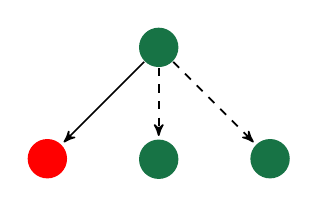
\begin{tikzpicture}[->,>=stealth',shorten >=1pt,auto,node distance=2cm,
                    semithick]
  \tikzstyle{every state}=[draw=none]

  \node[state, fill=darkspringgreen,minimum size=.5cm] 	     (A)                    {};
  \node[state, fill=red,minimum size=.5cm]         (B) [below left of=A] {};
  \node[state, fill=darkspringgreen,minimum size=.5cm]         (C) [below right of=A] {};
  \node[state, fill=darkspringgreen,minimum size=.5cm] 	     (D) [below =.9cm of A]                   {};

  \path[dashed] (A) edge              (D)
            	edge               (C);
  \path[->] (A) edge (B);

      \end{tikzpicture}
          \caption{Primary meristem transitioning to one vegetative meristem and generating two primary meristems.} 
  \end{subfigure}
            \hspace{\fill}  
  \begin{subfigure}[h]{.2\textwidth}
    \centering
      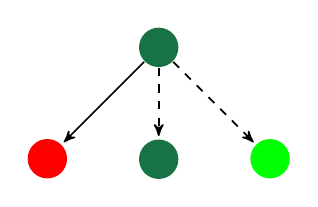
\begin{tikzpicture}[->,>=stealth',shorten >=1pt,auto,node distance=2cm,
                    semithick]
  \tikzstyle{every state}=[draw=none]

  \node[state, fill=darkspringgreen,minimum size=.5cm] 	     (A)                    {};
  \node[state, fill=red, minimum size=.5cm]         (B) [below left of=A] {};
  \node[state, fill=green, minimum size=.5cm]         (C) [below right of=A] {};
  \node[state, fill=darkspringgreen,minimum size=.5cm] 	     (D) [below =.9cm of A]                   {};

  \path[dashed] (A) edge              (D)
            	edge               (C);
  \path[->] (A) edge (B);

      \end{tikzpicture}
          \caption{Primary meristem transitioning to one vegetative meristem and generating primary and inflorescence meristems.} 
  \end{subfigure} 
              \hspace{\fill}
             \begin{subfigure}[h]{.2\textwidth}
    \centering
    \centering

      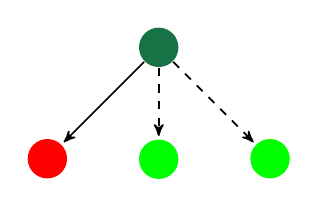
\begin{tikzpicture}[->,>=stealth',shorten >=1pt,auto,node distance=2cm,
                    semithick]
  \tikzstyle{every state}=[draw=none]

  \node[state, fill=darkspringgreen,minimum size=.5cm] 	     (A)                    {};
  \node[state, fill=red, minimum size=.5cm]         (B) [below left of=A] {};
  \node[state, fill=green, minimum size=.5cm]         (C) [below right of=A] {};
  \node[state, fill=green,minimum size=.5cm] 	     (D) [below =.9cm of A]                   {};

  \path[dashed] (A) edge              (D)
            	edge               (C);
  \path[->] (A) edge (B);

      \end{tikzpicture}
          \caption{Primary meristem transitioning to one vegetative meristem and generating inflorescence meristems.} 
  \end{subfigure} 
            \hspace{\fill}
  \begin{subfigure}[h]{.2\textwidth}
    \centering
    \centering
% stem cell expansion

% stem cell expansion
      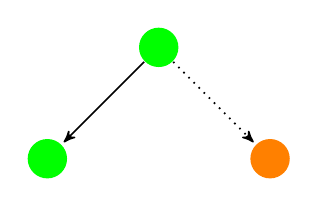
\begin{tikzpicture}[->,>=stealth',shorten >=1pt,auto,node distance=2cm,
                    semithick]
  %\tikzstyle{every state}=[fill=red,draw=none,text=white]

  \node[state, fill = green, draw = none,minimum size=.5cm] (A)                    {};
  \node[state, fill = green, draw = none,minimum size=.5cm]         (B) [below left of=A] {};
  \node[state, fill = orange, draw = none,minimum size=.5cm]         (C) [below right of=A] {};

  \path[dotted] (A) edge              (C);
  \path (A) edge		     (B);

      \end{tikzpicture}
    \caption{Inflorescence meristem remaining an inflorescence meristem and generating a floral meristem}
  \end{subfigure}\
        \caption{Meristem transitions in plants with indeterminate inflorescences.}
        \label{fig:transitions-indeterminate}
\end{figure}

\subsection*{Description of diagram}

The division shown in Figure \ref{fig:transitions-indeterminate}A occurs at rate $\beta_1 p(t)$. The rate is the product of $\beta_1$, the ..., and $p(t)$, the probability with which the division shown in Figure \ref{fig:transitions-indeterminate}A occurs. It results in the net gain of one primary meristem and gain of one vegetative meristem. The differential equations corresponding to this are:
%
\begin{align}
\dot{P} & = 2 \beta_1 p(t)  P - \beta_1 p(t) P = \beta_1 p(t) P \nonumber \\
\dot{V} & = \beta_1 p(t)  P      \nonumber \\
\dot{I} & = 0  \nonumber \\
\dot{F} & = 0
\end{align}
%
The division shown in Figure \ref{fig:transitions-indeterminate}B occurs at a rate $\beta_1 q(t)$. The rate is the product of $\beta_1$, the ..., and $q(t)$, the probability with which the division shown in Figure \ref{fig:transitions-indeterminate}B occurs. It results in the gain of one vegetative meristem and the gain of one inflorescence meristem. The differential equations corresponding to this are:
%
\begin{align}
\dot{P} & = 0 \nonumber \\
\dot{V} & = \beta_1 q(t) P      \nonumber \\
\dot{I} & =  \beta_1 q(t) P \nonumber \\
\dot{F} & = 0
\end{align}
%

The division shown in Figure \ref{fig:transitions-indeterminate}C occurs at a rate $\beta_1 r(t)$. The rate is the product of $\beta_1$, the ..., and $r(t)$, the probability with which the division shown in Figure \ref{fig:transitions-indeterminate}C occurs. It results in the net gain of two inflorescence meristems, gain of one vegetative meristem, and the loss of one primary meristem. The differential equations corresponding to this are:
%
\begin{align}
\dot{P} & = - \beta_1 r(t) P \nonumber \\
\dot{V} & = \beta_1 r(t)  P      \nonumber \\
\dot{I} & =  2 \beta_1 r(t) P \nonumber \\
\dot{F} & = 0
\end{align}
%

The division shown in Figure \ref{fig:transitions-indeterminate}D occurs at a rate $\beta_2 $. It results in the net gain of one floral meristem. The differential equations corresponding to this are:
%
\begin{align}
\dot{P} & = 0 \nonumber \\
\dot{V} & = 0      \nonumber \\
\dot{I} & =  0 \nonumber \\
\dot{F} & = \beta_2 I
\end{align}
%

The full system of differential equations for the system thus becomes:
%
\begin{align}
\dot{P} & = \beta_1 (p(t) - r(t)) P  \nonumber \\
\dot{V} & = \beta_1 (p(t) + q(t) + r(t) ) P     \nonumber \\
\dot{I} & =  \beta_1 (q(t) + 2 r(t) ) \nonumber \\
\dot{F} & = \beta_2 I
\end{align}
%
I assume that 
%
\begin{align}
p(t) + q(t) + r(t) \leq 1
\end{align}
Because they are probabilities, the controls $p(t)$, $q(t)$, and $r(t)$ are constrained on $[0,1]$. The difference between controls (e.g. $p(t) - r(t)$) is not constrained and can be negative. For example, when the probability of division into two inflorescence meristems is greater than the probability of division into two primary meristems, the value of $\dot{P}<0$ and corresponds to a decrease in the size of the primary meristem pool. If all primary meristem divisions are like in Panel A, $\dot{I} = 0$. If $p + q + r < 1$ at any point, than it's beneficial to increase p.

\end{document}
